% Created 2015-09-08 Tue 19:21
\documentclass[11pt]{article}
\usepackage[utf8]{inputenc}
\usepackage[T1]{fontenc}
\usepackage{fixltx2e}
\usepackage{graphicx}
\usepackage{longtable}
\usepackage{float}
\usepackage{wrapfig}
\usepackage{rotating}
\usepackage[normalem]{ulem}
\usepackage{amsmath}
\usepackage{textcomp}
\usepackage{marvosym}
\usepackage{wasysym}
\usepackage{amssymb}
\usepackage{capt-of}
\usepackage{hyperref}
\tolerance=1000
\usepackage[utf8]{inputenc}
\usepackage{commath}
\usepackage{pgf}
\usepackage{tikz}
\usetikzlibrary{shapes,backgrounds}
\usepackage{marginnote}
\usepackage{listings}
\usepackage{enumerate}
\usepackage{algpseudocode}
\usepackage{algorithm}
\usepackage{mathtools}
\usetikzlibrary{arrows,automata}
\setlength{\parskip}{16pt plus 2pt minus 2pt}
\renewcommand{\arraystretch}{1.6}
\DeclareMathOperator{\Neg}{Neg}
\author{Oleg Sivokon}
\date{\textit{<2015-09-07 Mon>}}
\title{Assignment 12, Authomata Theory}
\hypersetup{
 pdfauthor={Oleg Sivokon},
 pdftitle={Assignment 12, Authomata Theory},
 pdfkeywords={Automata Theory, Formal Languages, Assignment},
 pdfsubject={Second assignment in the course 20440 Automata and Formal Languages},
 pdfcreator={Emacs 25.0.50.1 (Org mode 8.3beta)}, 
 pdflang={English}}
\begin{document}

\maketitle
\tableofcontents

\definecolor{codebg}{rgb}{0.96,0.99,0.8}
\definecolor{codestr}{rgb}{0.46,0.09,0.2}
\lstset{%
  backgroundcolor=\color{codebg},
  basicstyle=\ttfamily\scriptsize,
  breakatwhitespace=false,
  breaklines=false,
  captionpos=b,
  framexleftmargin=10pt,
  xleftmargin=10pt,
  framerule=0pt,
  frame=tb,
  keepspaces=true,
  keywordstyle=\color{blue},
  showspaces=false,
  showstringspaces=false,
  showtabs=false,
  stringstyle=\color{codestr},
  tabsize=2
}
\lstnewenvironment{maxima}{%
  \lstset{%
    backgroundcolor=\color{codebg},
    escapeinside={(*@}{@*)},
    aboveskip=20pt,
    captionpos=b,
    label=,
    caption=,
    showstringspaces=false,
    frame=single,
    framerule=0pt,
    basicstyle=\ttfamily\scriptsize,
    columns=fixed}}{}
}
\makeatletter
\newcommand{\verbatimfont}[1]{\renewcommand{\verbatim@font}{\ttfamily#1}}
\makeatother
\verbatimfont{\small}%
\clearpage

\section{Problems}
\label{sec:orgheadline17}

\subsection{Problem 1}
\label{sec:orgheadline4}
\begin{enumerate}
\item Build an NFA for the language over alphabet \(\{a,b\}\) where words must
start with \(bab\) and end in \(b\).
\item Build an NFA for the language over alphabet \(\{a,b,c\}\), defined as
follows: \(L = \{w \;|\; \exists n,m,k \in \mathbb{N}.(w = a^nb^mc^k \land
      \#(w) \mod 2 = 0)\}\).
\item Build an NFA for the language over alphabet \(\{a,b\}\), s.t. it contains
all words with substring \(aba\) repeated at least twice.
\end{enumerate}

\subsubsection{Answer 1}
\label{sec:orgheadline1}
\begin{tikzpicture}[->,>=stealth',shorten >=1pt,auto,node distance=2.8cm,
                    semithick]

  \node[initial,state]   (A)              {$q_0$};
  \node[state]           (B) [right of=A] {$q_1$};
  \node[state]           (C) [right of=B] {$q_2$};
  \node[accepting,state] (D) [right of=C] {$q_3$};
  \node[state]           (E) [below of=D] {$q_4$};

  \path (A) edge              node {b} (B)
        (B) edge              node {a} (C)
        (C) edge              node {b} (D)
        (D) edge              node {a} (E)
            edge [loop above] node {b} (D)
        (E) edge              node {b} (D)
            edge [loop right] node {a} (E);
\end{tikzpicture}

\emph{The nodes where automaton dies are not shown.}

The language accepted by this automaton must start with the prefix \(bab\) as
can be seen in diagram above.  The only accepting state has transitions
pointing at it only on inputs \(b\), thus all words accepted by this language
must end in \(b\).

Conversely, if the words start with the prefix \(bab\), then we must reach the
statate \(\hat{\delta}(bab, q_0) = q_4\).  From \(q_4\) the input can be either
accepted, since it already ends in any number of \(b\), or it may follow
through to \(q_4\) and whenever \(b\) is encountered in the input---return to
\(q_3\).  Since all execution path will thus lead to the accepting state on
\(b\) or to rejecting state on \(a\), I conclude that all words with prefix \(bab\)
and ending in \(b\) are accepted by the described automaton.

\subsubsection{Answer 2}
\label{sec:orgheadline2}
A regular expression to summarize the effort: \((((aa)^*((bb)^*(cc)^*) +
    (b(bb)^*c(cc)^*))) + (a(aa)^*((b(bb)^*(cc)^*) + (b(bb)^*(cc)^*)))\).

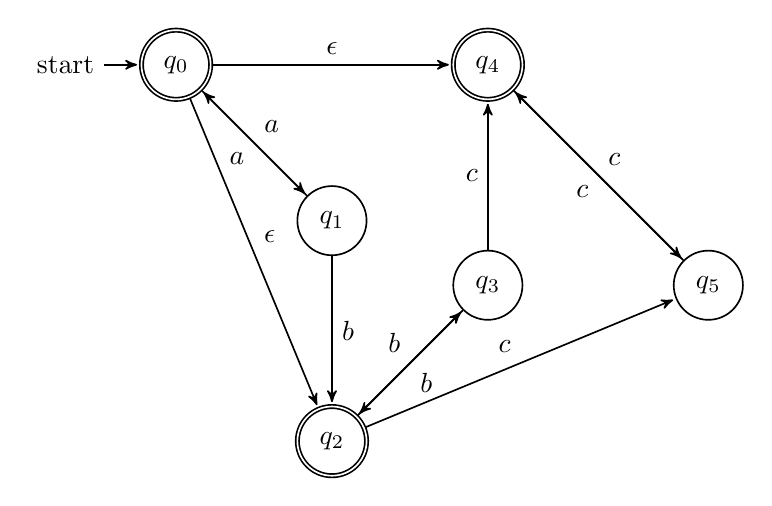
\begin{tikzpicture}[->,>=stealth',shorten >=1pt,auto,node distance=2.8cm,
                    semithick]

  \node[accepting,initial,state]   (A)              {$q_0$};
  \node[state]                     (B) [below right of=A] {$q_1$};
  \node[accepting,state]           (C) [below of=B] {$q_2$};
  \node[state]                     (D) [above right of=C] {$q_3$};
  \node[accepting,state]           (E) [above of=D] {$q_4$};
  \node[state]                     (F) [right of=D] {$q_5$};

  \path (A) edge node {$a$}        (B)
            edge node {$\epsilon$} (C)
            edge node {$\epsilon$} (E)
        (B) edge node {$a$}        (A)
            edge node {$b$}        (C)
        (C) edge node {$b$}        (D)
            edge node {$c$}        (F)
        (D) edge node {$b$}        (C)
            edge node {$c$}        (E)
        (E) edge node {$c$}        (F)
        (F) edge node {$c$}        (E);
\end{tikzpicture}

Essentially, what happens in this diagram is as follows:
\begin{enumerate}
\item On first input we decide whether the prefix starts with \(a\), \(b\) or \(c\).
\item Once decided, we parse more of the prefix.
\begin{itemize}
\item If the prefix was \(c\), we make sure there is even number of \(c\).
\item If the prefix started with \(b\), we create two branches, one will pick
the non-accepting state of the bit of automaton processing \(c\) prefix
once we counted even number of \(b\) inputs, and an accepting state
otherwise.
\item If our prefix was \(a\), then we will proceed similarly to the previous
case, however, we will switch roles: on odd number of \(a's\), we will
switch to an accepting state and to a non-accepting state otherwise.
\end{itemize}
\end{enumerate}

\subsubsection{Answer 3}
\label{sec:orgheadline3}
The diagram below can be also given by the regular expression:
\(((ab)^*b^*)^*aba(ba + (((ab)^*b^*)aba))(a + b)^*\).  An easier, but a
sloppier way to write the same regexp would be:
\((a + b)^*(ababa + (aba(a + b)^*aba))(a + b)^*\).

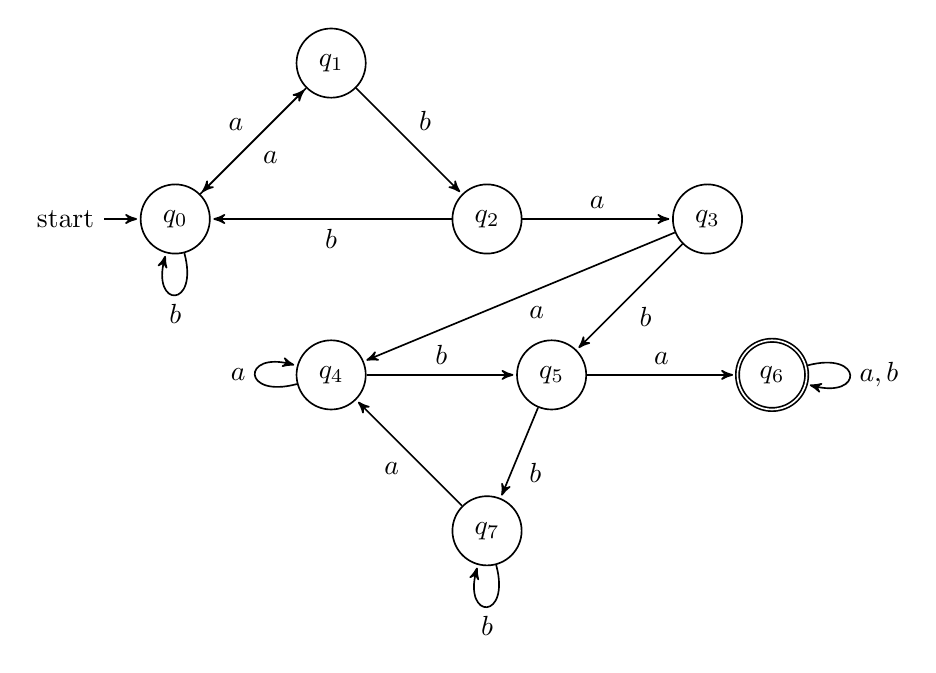
\begin{tikzpicture}[->,>=stealth',shorten >=1pt,auto,node distance=2.8cm,
                    semithick]

  \node[initial,state]   (A)                    {$q_0$};
  \node[state]           (B) [above right of=A] {$q_1$};
  \node[state]           (C) [below right of=B] {$q_2$};
  \node[state]           (D) [right of=C]       {$q_3$};
  \node[state]           (E) [below left of=C]  {$q_4$};
  \node[state]           (F) [below left of=D]  {$q_5$};
  \node[accepting,state] (G) [right of=F]       {$q_6$};
  \node[state]           (H) [below right of=E] {$q_7$};

  \path (A) edge [loop below] node {$b$}   (B)
            edge              node {$a$}   (B)
        (B) edge              node {$a$}   (A)
            edge              node {$b$}   (C)
        (C) edge              node {$a$}   (D)
            edge              node {$b$}   (A)
        (D) edge              node {$a$}   (E)
            edge              node {$b$}   (F)
        (E) edge [loop left]  node {$a$}   (E)
            edge              node {$b$}   (F)
        (F) edge              node {$a$}   (G)
            edge              node {$b$}   (H)
        (G) edge [loop right] node {$a,b$} (G)
        (H) edge              node {$a$}   (E)
            edge [loop below] node {$b$}   (E);
\end{tikzpicture}

Put in words: skip over repetitions of \(bb\) possibly preceded by \(a\), until
encountering \(aba\) substring.  Once that happens, consider the prefix of the
second \(aba\) substring found.  If the next input is \(b\), continue matching,
else---bail out and essentially repeat the previously described procedure.

\subsection{Problem 2}
\label{sec:orgheadline8}
Prove or disprove that pairs of regular expressions to follow accept the same
language.
\begin{enumerate}
\item \((0(10^*)^*)^*+1^*\) and \((1+0)^*\).
\item \((1+0)^+\) and \((0^*1)^*(1^*0)^++(0^*1)^+\).
\item \(1^*(0^*10^*)^*\) and \((101^*)^*1^*\).
\end{enumerate}

\subsubsection{Answer 3}
\label{sec:orgheadline5}
Two expressions are not equivalent.  \((1+0)^*\) matches any binary string,
while \((0(10^*)^*)^*+1^*\) doesn't match any binary string containing with a
prefix 00 or more consequtive zeros.

\subsubsection{Answer 4}
\label{sec:orgheadline6}
Two expressions are equivalent.  \((0^*1)^+\) will match any binary at least
one character long string edning in 1, while \((1^*0)^+\) will match any
binary string at least one character long ending in 0.  The union of these
two expressions will match all binary strings of length at least 1, which is
equivalent to \((1+0)^+\).  The \((0^*1)^*\) of the second expression plays no
role (is redundant).

\subsubsection{Answer 5}
\label{sec:orgheadline7}
Teo expressions are not equivalent.  \((101^*)^*1^*\) will not match string
containing 00 or more consequent zeros as a substring, while this is not a
problem for \(1^*(0^*10^*)^*\).

\subsection{Problem 3}
\label{sec:orgheadline10}
Write a regular expression for the language over alphabet \(\{a,b\}\) s.t. all
words in this language start with either \(aa\) or \(bbb\) and none of them
contains substring \(bab\).

\subsubsection{Answer 6}
\label{sec:orgheadline9}
The desired regex is \((bbb^+)^*(aa^+b^*)^*\).

\subsection{Problem 4}
\label{sec:orgheadline11}
Write an algorithm which accepts a regular expression \(r\) and produces a
language \(\overline{L[r]}\).

\subsection{Problem 5}
\label{sec:orgheadline13}
Build a DFA from given NFA:

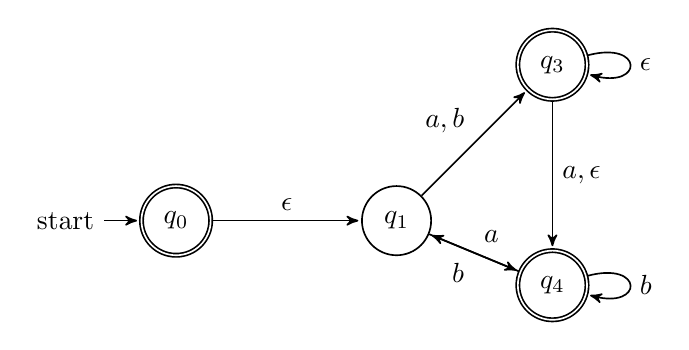
\begin{tikzpicture}[->,>=stealth',shorten >=1pt,auto,node distance=2.8cm,
                    semithick]

  \node[accepting,initial,state]   (A)                    {$q_0$};
  \node[state]                     (B) [right of=A]       {$q_1$};
  \node[accepting,state]           (C) [above right of=B] {$q_3$};
  \node[accepting,state]           (D) [below of=C]       {$q_4$};

  \path (A) edge              node {$\epsilon$}   (B)
        (B) edge              node {$a,b$}        (C)
            edge              node {$a$}          (D)
        (C) edge [loop right] node {$\epsilon$}   (D)
            edge              node {$a,\epsilon$} (D)
        (D) edge              node {$b$}          (B)
            edge [loop right] node {$b$}          (D);
\end{tikzpicture}

\subsubsection{Answer 7}
\label{sec:orgheadline12}
The corresponding DFA can be written as:

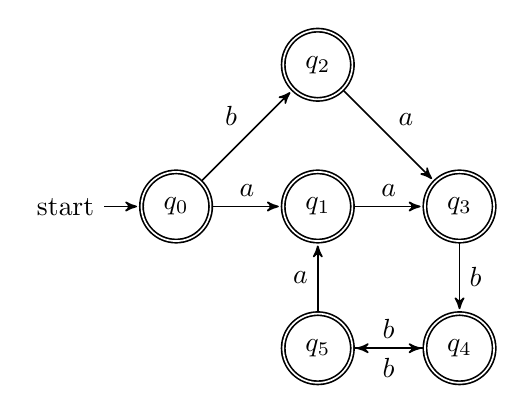
\begin{tikzpicture}[->,>=stealth',shorten >=1pt,auto,node distance=1.8cm,
                    semithick]

  \node[accepting,initial,state]   (A)              {$q_0$};
  \node[accepting,state]           (B) [right of=A] {$q_1$};
  \node[accepting,state]           (C) [above of=B] {$q_2$};
  \node[accepting,state]           (D) [right of=B] {$q_3$};
  \node[accepting,state]           (E) [below of=D] {$q_4$};
  \node[accepting,state]           (F) [left of=E]  {$q_5$};

  \path (A) edge  node {$a$}   (B)
            edge  node {$b$}   (C)
        (B) edge  node {$a$}   (D)
        (C) edge  node {$a$}   (D)
        (D) edge  node {$b$}   (E)
        (E) edge  node {$b$}   (F)
        (F) edge  node {$b$}   (E)
            edge  node {$a$}   (B);
\end{tikzpicture}

\emph{Nodes where automata dies are not shown.}

\subsection{Problem 6}
\label{sec:orgheadline15}
Write a regular expression for the diagram below:

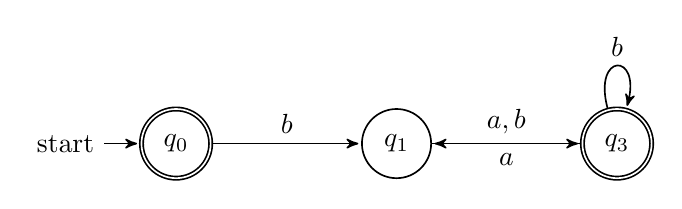
\begin{tikzpicture}[->,>=stealth',shorten >=1pt,auto,node distance=2.8cm,
                    semithick]

  \node[accepting,initial,state]   (A)              {$q_0$};
  \node[state]                     (B) [right of=A] {$q_1$};
  \node[accepting,state]           (C) [right of=B] {$q_3$};

  \path (A) edge              node {$b$}   (B)
        (B) edge              node {$a,b$} (C)
        (C) edge [loop above] node {$b$}   (D)
            edge              node {$a$}   (B);
\end{tikzpicture}

\emph{Nodes where the automata dies are not shown.}

\subsubsection{Answer 8}
\label{sec:orgheadline14}
The regular expression for the diagram above: \(\epsilon + b((a + b)b^*)^+\).

\subsection{Problem 7}
\label{sec:orgheadline16}
Given regular expression \(r\) and \(L\), a language over \(\Sigma\) which
designates regular expression \(r\Sigma^*\).  Prove that unless \(L = \Sigma^*\)
and \(L = \emptyset\), there doesn't exist a regular expression \(s\) s.t.
\(s\Sigma^*\) designates \(\overline{L}\).
\end{document}